\section{Neural activation prior}
\label{sec:nap}
Our NAP is based on the following observation for OOD detection:
for a channel located before the global pooling layer in a fully trained neural network, the likelihood that a small number of its neurons activated with a stronger response to an ID sample is significantly higher compared to an OOD sample. For the behavior in other layers of the neural network, refer to the discussion around Figure~\ref{fig:max-mean} in Section~\ref{sec:does}. 

To formally describe this observation, we first define the concept of neural activation. 
Consider a trained classification neural network \( f \), assuming it receives \( D \)-dimensional input \( x \) and outputs \( K \)-dimensional logits. That is \( f: \mathbb{R}^D \rightarrow \mathbb{R}^K \). We concentrate on the activation tensor \( \mathbf{A} \) , located at the penultimate layer just before the global pooling operation, as illustrated in Figure~\ref{fig:pos}. Let the dimensions of \( \mathbf{A} \) be \( C \times H \times W \), where \( C \) is the number of channels, and \( H \) and \( W \) are the spatial dimensions.

\begin{figure}[!h]
% \vspace{-9pt}
  \centering
  \begin{subfigure}{0.49\linewidth}
    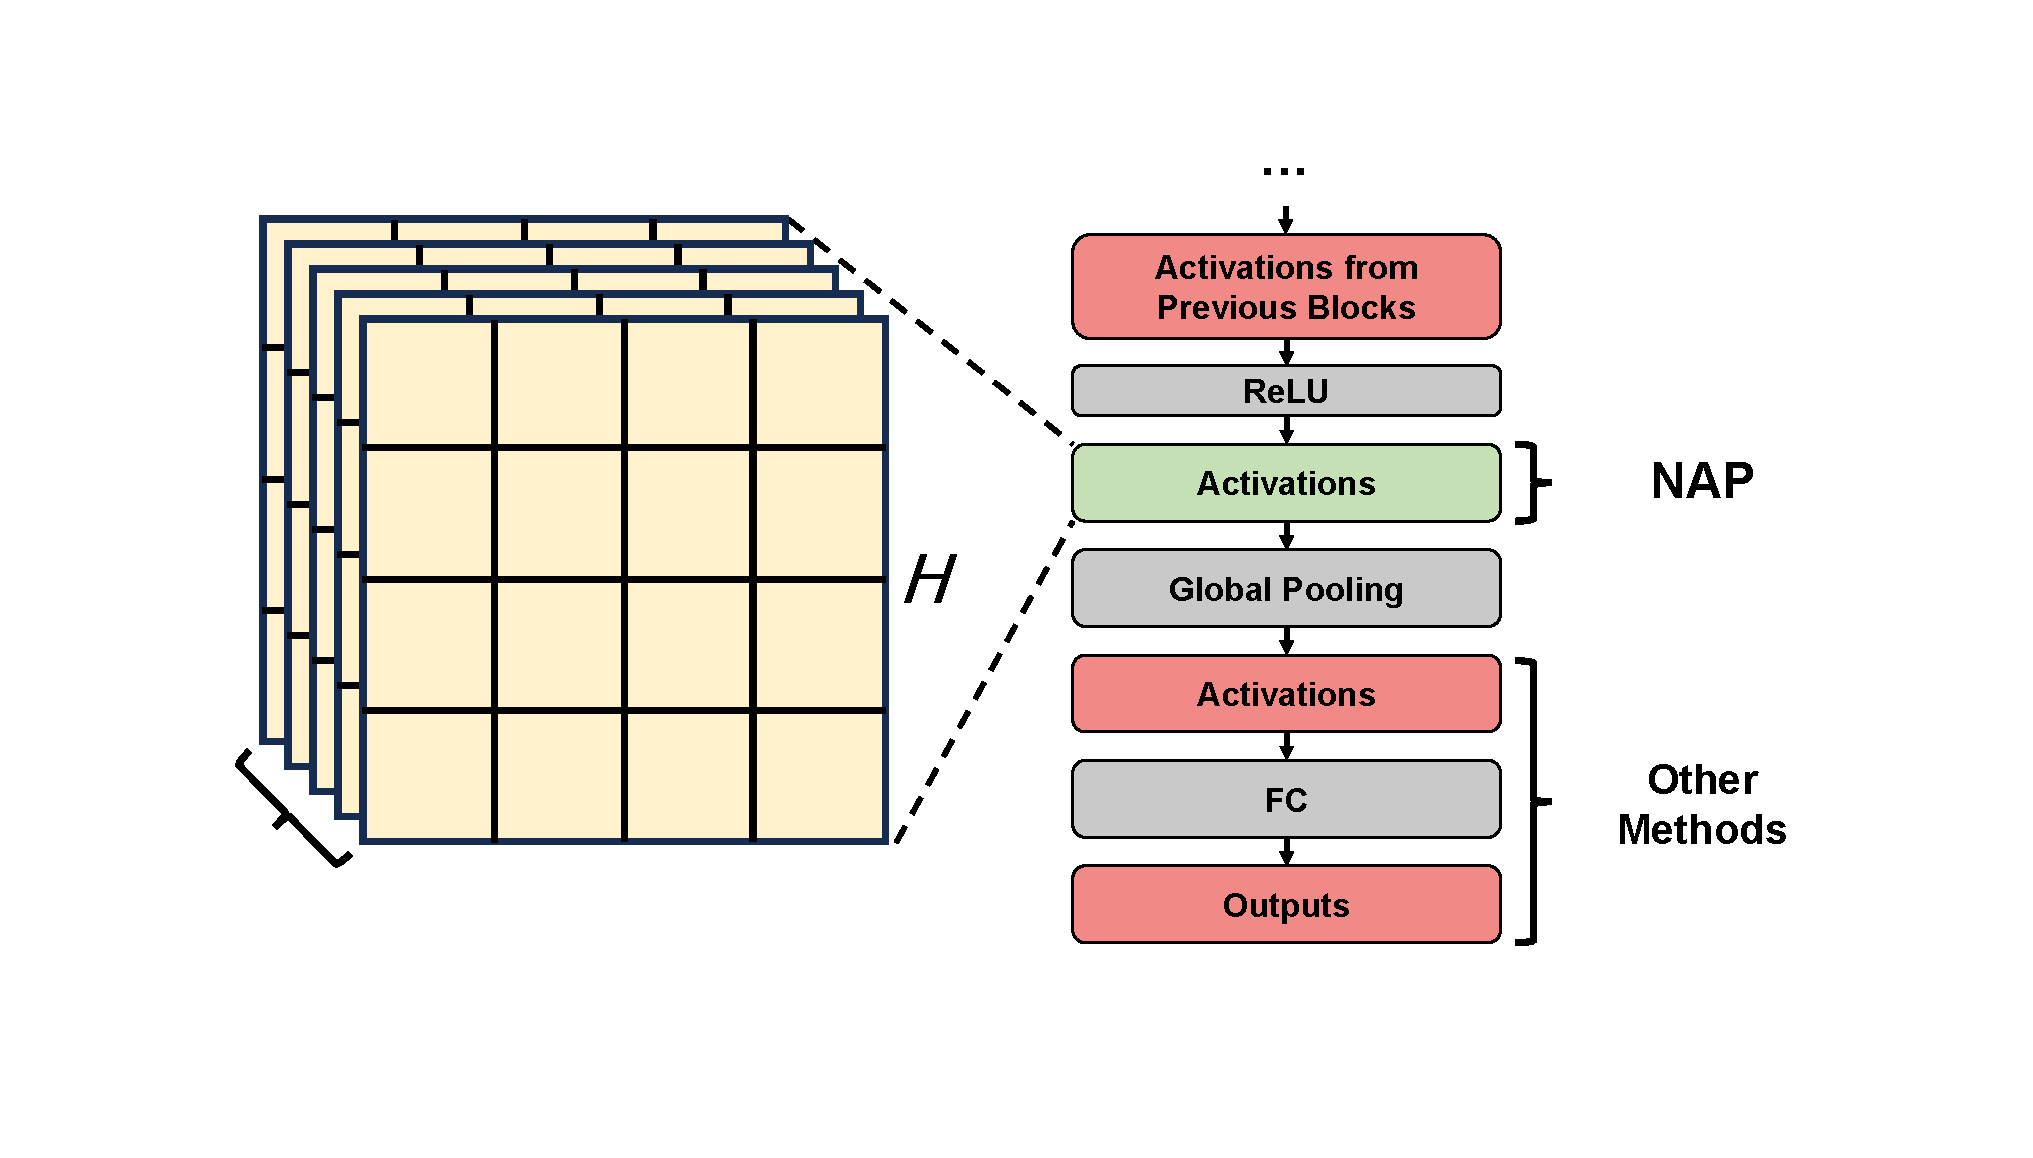
\includegraphics[width=\linewidth]{eps/CNN-pos.eps}
    \caption{NAP in CNN}
    \label{fig:pos}
  \end{subfigure}
  \hfill
  \begin{subfigure}{0.49\linewidth}
    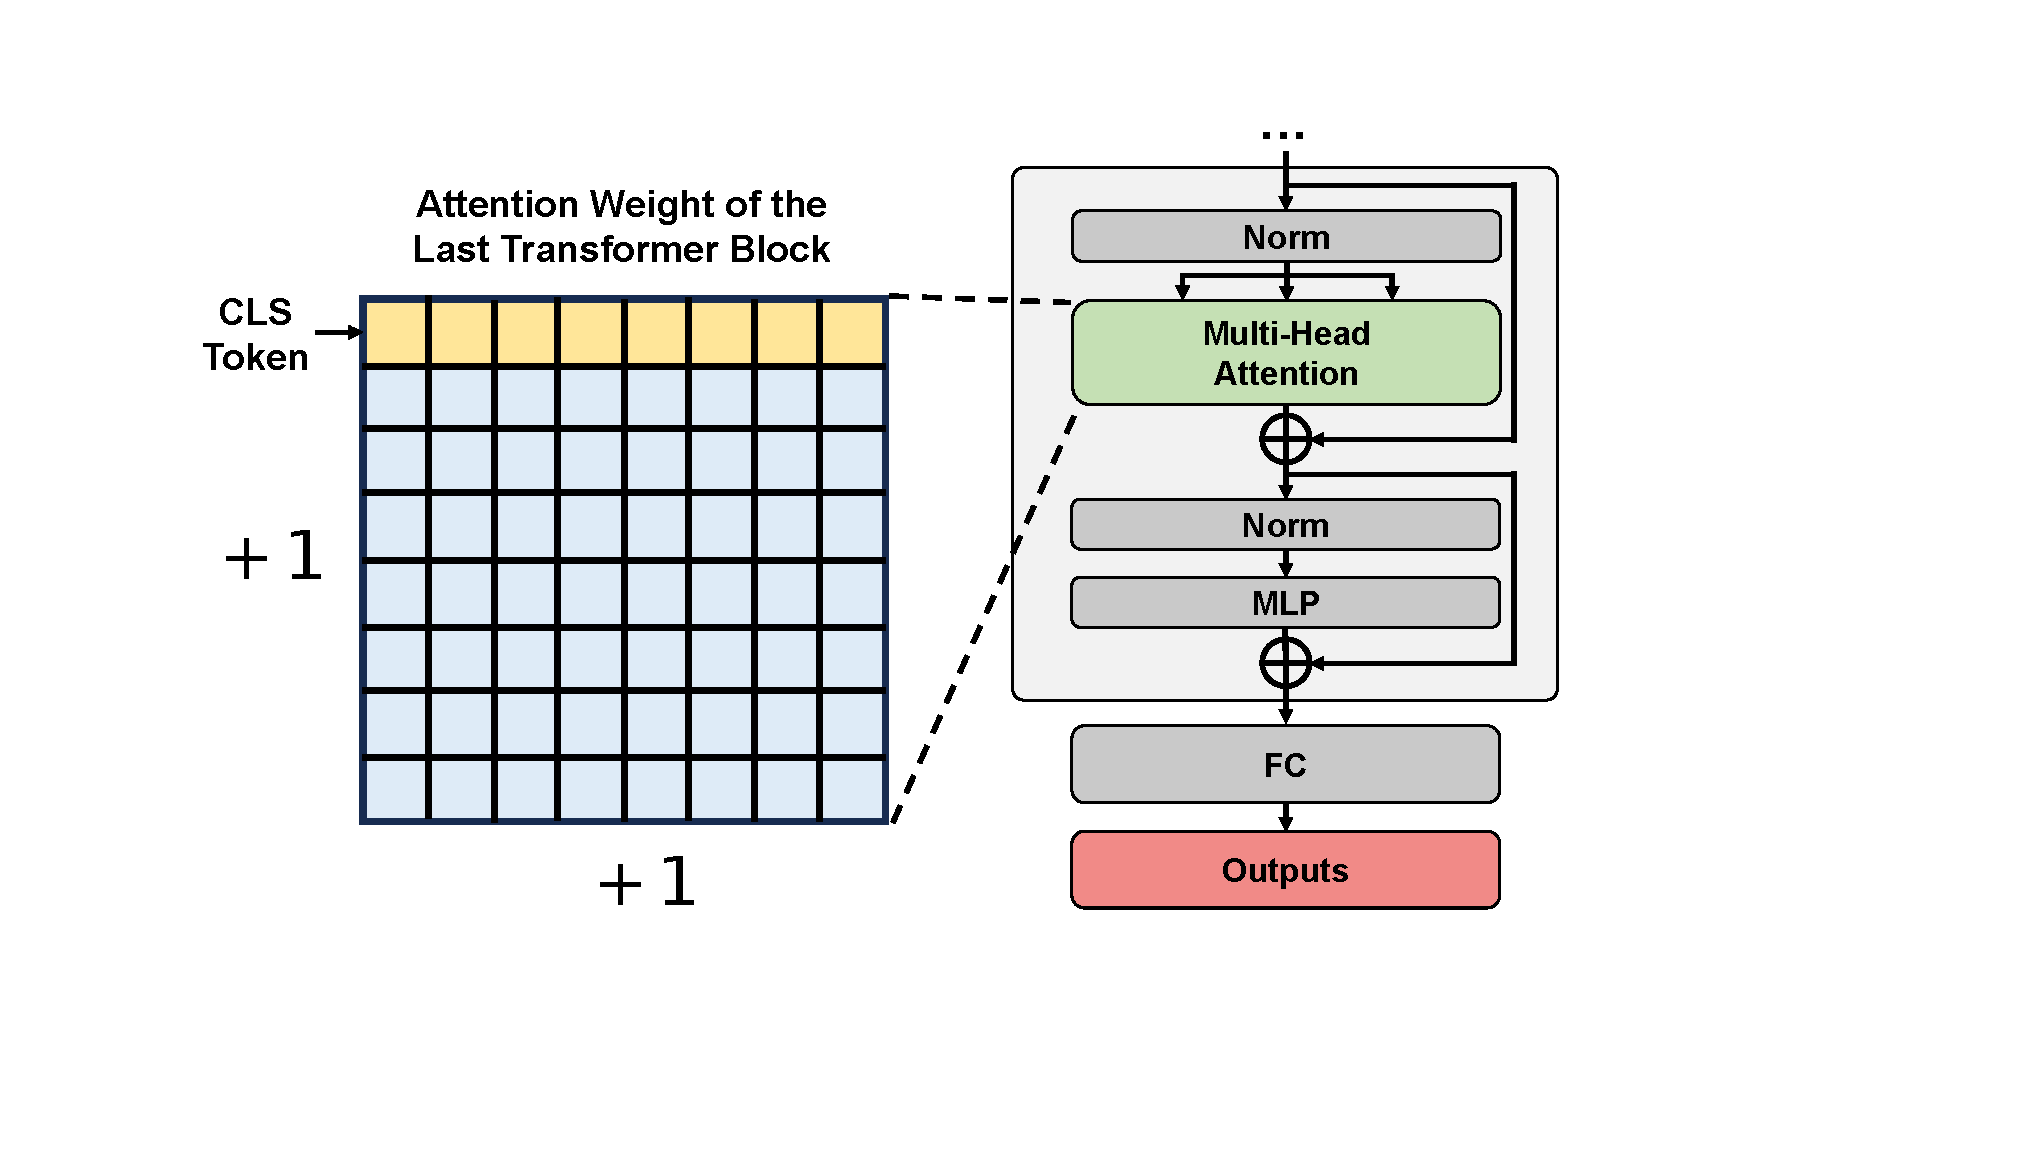
\includegraphics[width=\linewidth]{eps/ViT-pos.eps}
    \caption{NAP in Transformer}
    \label{fig:vit}
  \end{subfigure}
  \caption{\textbf{Illustration identifying the focus zone of Neural Activation Prior (NAP) in classification neural networks.} The figure highlights the specific position of NAP in the network: (a) For the CNN-based model, the activation value in the green part is the location of the NAP proposed in this article, which is before global pooling. (b) For the Transformer model, NAP is highlighted within the cls token's attention weights in the last Transformer block, illustrating a targeted approach in contrast to most existing methods that focus on regions after global pooling.}
  \label{fig:pos-both}
  % \vspace{-9pt}
\end{figure}

Let \( \mathbf{A}_j \) represent the activation tensor of the \( j \)-th channel. We define two key statistical indicators of \( \mathbf{A}_j \) as follows:
\begin{itemize}
\item \textbf{Maximum activation value:}
\begin{equation}
\text{Max}(\mathbf{A}_j) = \max_{k,l} \mathbf{A}_{jkl},
\end{equation}
where \( \text{Max}(\mathbf{A}_j) \) is the maximum value among all elements in the activation vector \( \mathbf{A}_j \). Here, \( k \) and \( l \) index the spatial dimensions (height and width) of the activation map, respectively. Notice that $\mathbf{A}_{jkl}$ is processed by ReLU (as shown in Figure~\ref{fig:pos}), hence $\mathbf{A}_{jkl}\geq0$.
% comment: relu
\item \textbf{Mean activation value:}
\begin{equation}
\text{Mean}(\mathbf{A}_j) = \frac{1}{h \times w} \sum_{k=1}^{h} \sum_{l=1}^{w} \mathbf{A}_{jkl},
\end{equation}
where \( \text{Mean}(\mathbf{A}_j) \) is the average of all activation values in the \( j \)-th channel.

\end{itemize}

Inspired by the concept of signal-to-noise ratio, we interpret \( \text{Max}(\mathbf{A}_j) \) as the signal strength and \( \text{Mean}(\mathbf{A}_j) \) as the noise strength. The ratio of these values can be viewed as an indicator of the quality of the activation vector \( \mathbf{A}_j \). Note that we calculate this metric separately for each channel in the network, since different channels are usually used to detect different patterns. In the context of OOD detection, this quality measure can be used to assess whether the neural network recognizes the input sample --- in other words, this measure can be used to judge whether a sample is within the training set distribution. As shown in Figure~\ref{fig:one}, this phenomenon is termed as the neural activation prior.

It is worth noting that our proposed prior is orthogonal to existing OOD detection methods. As illustrated in Figure~\ref{fig:pos}, existing methods mainly focus on the network output and weight of the penultimate layer after global pooling, and leverage them to design various scoring functions for OOD detection. In contrast, the prior we propose focuses on the channels of the penultimate layer before global pooling. Since the distribution information within these channels is inevitably lost during the global pooling process, our proposed prior is complementary to existing work. 

\noindent \textbf{Extension to Transformer backbones.} We observe that the classify (cls) token in the last block of Transformers can be effectively utilized as an analogue to the pooled activations used in CNNs for our method. Consequently, as illustrated in Figure~\ref{fig:vit}, we calculate NAP score by employing the attention vectors associated with the \textbf{cls} token from the final Transformer block. This approach mirrors our methodological framework in CNNs, facilitating a coherent extension across both architectures. The specifics of the scoring function for NAP, applicable to both CNNs and Transformers, will be further elucidated in Section~\ref{sec:scoring}.